\section{Evaluation}
\label{sec:evaluation}

% \vv{estes testes incluem o tempo de parsing? nao deveriam. deveriam só
%   contar o tempo da chamada à funcao bisimilar/equivalent.}

We implemented the algorithm skteched in Listings~\ref{lst:toGrammar}
to~\ref{lst:enhanced} in 300 lines of Haskell and used the Glasgow
Haskell Compiler, GHC version 8.6.3, from which we have obtained the
results we present in this section.  Evaluation was conducted on a Mac
mini equipped with a 3.6 GHz Intel Core i3, 8 GB of memory, running
MacOS 10.14.3.

Once the improvement proposals were established, we benchmarked the
algorithm on a test suite of carefully crafted pair of types. These
tests comprise valid and invalid equivalences, for a total of 138
tests. We have profiled our program for the time and memory allocated
during the tests. For this purpose, we have used GHC's profiling
feature, that maintains a cost-centre stack to keep track of the
incurred costs. We ran the tests 10 times, kept a record of the run
time and memory allocated for each run, discarded the best and worst
values obtained and, then, we have measured the average of the
remaining values. The results are depicted in
Figure~\ref{fig:results}.

\begin{figure}[h]
	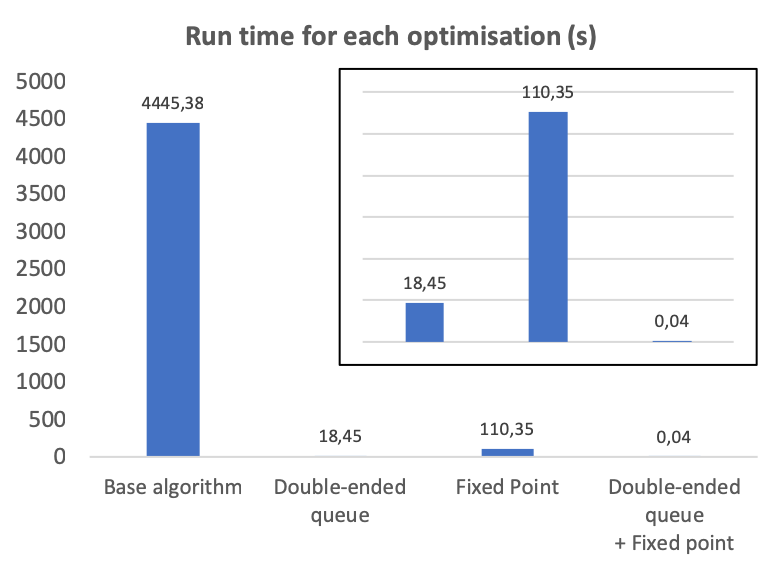
\includegraphics[height=5cm]{img/run_time}	\enspace
	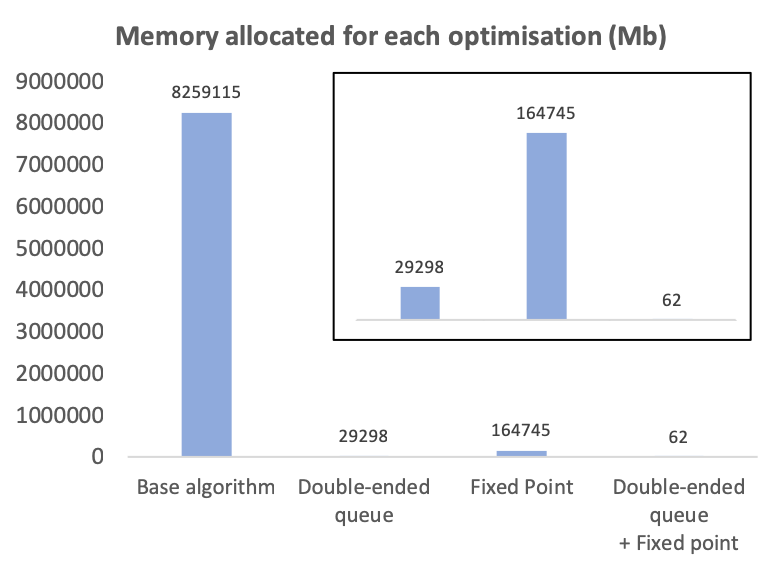
\includegraphics[height=5cm]{img/memory_alloc}
	\caption{Test results: running times (on the left) and
	memory allocated (on the right) checking the equivalence
	of context-free session types in 138 tests.}
	\label{fig:results}
\end{figure}

For the base algorithm, proposed in Listing~\ref{lst:algorithm}, we
obtained an average running time of about 4445.38 seconds and
8,259,115 Mb memory allocated. From the moment we introduced the
optimizations the results improved remarkably: iterating the
simplification phase in the search for a fixed point allowed to reduce
the running time to 110.35 seconds and the memory allocated to 164,745
Mb, whereas the implementation of the double-ended queue allowed to
reduce the running time to 18.45 seconds and the allocated memory to
29,298. The combination of both exhibit an improvement on more than
12,000,000\% from the base case, achieving an average of 0.04
seconds for the running time and 62 Mb of allocated memory.

We should also highlight that, we run example~\eqref{ex:chaotic}
with the improved algorithm, in a battery os 100 runs, and obtained an
average running time of 0.008 seconds.

The heuristic we proposed actually circumvents the exponential complexity 
inherent to the expansion tree, thus allowing to obtain running times that 
are manifestly small, thus allowing the use of this algorithm as an integral 
part of a compiler, as we had intended from the beginning.

%%% Local Variables:
%%% mode: latex
%%% TeX-master: "main"
%%% End:
